\documentclass[aspectratio=169,11pt]{beamer}

% =========================================================
% Theme
% =========================================================
\usetheme{Madrid}
\usecolortheme{seahorse}
\setbeamertemplate{navigation symbols}{}

% =========================================================
% Packages
% =========================================================
\usepackage[utf8]{inputenc}
\usepackage[T1]{fontenc}
\usepackage{lmodern}
\usepackage{amsmath,amssymb}
\usepackage{xcolor}
\usepackage{booktabs}
\usepackage{array}
\usepackage{listings}
\usepackage{tikz}
\usetikzlibrary{arrows.meta,positioning,fit,calc,shapes.geometric}
\usepackage{hyperref}
\hypersetup{pdfpagemode=UseNone}

% =========================================================
% Colors
% =========================================================
\definecolor{deepblue}{RGB}{0,51,102}
\definecolor{softblue}{RGB}{220,235,247}
\definecolor{softgreen}{RGB}{223,242,228}
\definecolor{softorange}{RGB}{255,238,214}
\definecolor{softred}{RGB}{252,228,228}
\definecolor{codebg}{RGB}{248,248,248}
\definecolor{mygray}{RGB}{90,90,90}
\definecolor{mypurple}{RGB}{102,0,153}

% =========================================================
% Listings
% =========================================================
\lstset{
	language=Java,
	basicstyle=\ttfamily\small,
	backgroundcolor=\color{codebg},
	frame=single,
	breaklines=true,
	columns=fullflexible,
	showstringspaces=false,
	keywordstyle=\color{deepblue}\bfseries,
	commentstyle=\color{green!50!black},
	stringstyle=\color{mypurple},
	numbers=left,
	numberstyle=\tiny\color{mygray},
	stepnumber=1,
	numbersep=8pt
}

% =========================================================
% Title Info
% =========================================================
\title[Week 4 -- Part 2]{Concurrency and Distributed Systems}
\subtitle{Week 4 -- Part 2: \texttt{volatile} and Happens-Before}
\author{Dr. Mohamad Aoude}
\institute{Faculty of Engineering}
\date{\today}

% =========================================================
% Custom Blocks
% =========================================================
\setbeamercolor{block title}{bg=deepblue!85, fg=white}
\setbeamercolor{block body}{bg=softblue, fg=black}

\setbeamercolor{alertblock title}{bg=red!75!black, fg=white}
\setbeamercolor{alertblock body}{bg=softred, fg=black}

\setbeamercolor{exampleblock title}{bg=green!50!black, fg=white}
\setbeamercolor{exampleblock body}{bg=softgreen, fg=black}

% =========================================================
% Footer
% =========================================================
\setbeamertemplate{footline}{
	\leavevmode
	\hbox{
		\begin{beamercolorbox}[wd=.78\paperwidth,ht=2.5ex,dp=1.2ex,leftskip=0.3cm]{author in head/foot}
			\usebeamerfont{author in head/foot}Concurrency and Distributed Systems --- Week 4 Part 2
		\end{beamercolorbox}
		\begin{beamercolorbox}[wd=.22\paperwidth,ht=2.5ex,dp=1.2ex,rightskip=0.3cm]{date in head/foot}
			\hfill \insertframenumber/\inserttotalframenumber
		\end{beamercolorbox}
	}
}

% =========================================================
% Document
% =========================================================
\begin{document}
	
	% =========================================================
	\begin{frame}
		\titlepage
	\end{frame}
	
	% =========================================================
	\begin{frame}{Part 2 Roadmap}
		\tableofcontents
	\end{frame}
	
	\section{From Visibility Problem to Visibility Tool}
	\section{The Meaning of volatile}
	\section{Visibility and Ordering}
	\section{Happens-Before}
	\section{Publication Patterns}
	\section{Why volatile Is Not Atomic}
	\section{Lab Preparation}
	
	% =========================================================
	\begin{frame}{Where We Are in Week 4}
		\begin{block}{Part 1}
			We learned that unsynchronized shared variables are not reliable communication channels:
			\begin{itemize}
				\item stale reads can happen
				\item threads may observe different values
				\item the Java Memory Model defines what is allowed
			\end{itemize}
		\end{block}
		
		\vspace{0.3cm}
		
		\begin{block}{Part 2}
			Now we study the first explicit memory-visibility tool:
			\[
			\texttt{volatile}
			\]
			and the key formal relation:
			\[
			\textbf{happens-before}
			\]
		\end{block}
		
		\vspace{0.3cm}
		
		\begin{exampleblock}{Main transition}
			Part 1 answered: \emph{Why can visibility fail?}
			
			Part 2 answers: \emph{How can Java establish visibility and ordering guarantees?}
		\end{exampleblock}
	\end{frame}
	
	% =========================================================
	\begin{frame}{Learning Objectives}
		By the end of this lecture, students should be able to:
		
		\begin{itemize}
			\item explain what \texttt{volatile} guarantees
			\item explain what \texttt{volatile} does \emph{not} guarantee
			\item distinguish visibility from atomicity
			\item explain, in practical terms, the meaning of \textbf{happens-before}
			\item identify simple publication patterns using a volatile flag
			\item connect \texttt{volatile} to ordering constraints
			\item understand why \texttt{volatile} cannot fix \texttt{counter++}
		\end{itemize}
	\end{frame}
	
	% =========================================================
	\begin{frame}[fragile]{Return to the Stop-Flag Problem}
		\begin{lstlisting}
			class StopDemo {
				static boolean running = true;
				
				public static void main(String[] args) throws Exception {
					Thread worker = new Thread(() -> {
						while (running) {
							// busy wait
						}
						System.out.println("Worker stopped");
					});
					
					worker.start();
					Thread.sleep(1000);
					running = false;
				}
			}
		\end{lstlisting}
		
		\vspace{0.2cm}
		
		\begin{alertblock}{Problem}
			There is no formal guarantee that the worker will observe the write promptly.
		\end{alertblock}
	\end{frame}
	
	% =========================================================
	\begin{frame}[fragile]{Fixing the Communication Variable}
		\begin{lstlisting}
			class StopDemoFixed {
				static volatile boolean running = true;
				
				public static void main(String[] args) throws Exception {
					Thread worker = new Thread(() -> {
						while (running) {
							// busy wait
						}
						System.out.println("Worker stopped");
					});
					
					worker.start();
					Thread.sleep(1000);
					running = false;
				}
			}
		\end{lstlisting}
		
		\vspace{0.2cm}
		
		\begin{exampleblock}{What changed?}
			The variable is no longer an ordinary shared field.  
			It now has special memory-visibility semantics.
		\end{exampleblock}
	\end{frame}
	
	% =========================================================
	\begin{frame}{What \texttt{volatile} Means}
		\begin{block}{Practical definition}
			A \texttt{volatile} variable is a shared variable whose reads and writes participate in stronger memory-visibility and ordering rules.
		\end{block}
		
		\vspace{0.3cm}
		
		When one thread writes a new value to a volatile variable:
		\begin{itemize}
			\item other threads are required to observe that write correctly through later volatile reads
			\item certain reorderings around that access are restricted
		\end{itemize}
		
		\vspace{0.3cm}
		
		\begin{alertblock}{Important}
			\texttt{volatile} is not a lock.  
			It does not make threads take turns.
		\end{alertblock}
	\end{frame}
	
	% =========================================================
	\begin{frame}{The Two Core Guarantees of volatile}
		\begin{columns}[T]
			\column{0.48\textwidth}
			\begin{block}{1. Visibility}
				A write to a volatile variable by one thread becomes visible to later reads of that same variable by another thread.
			\end{block}
			
			\column{0.48\textwidth}
			\begin{block}{2. Ordering}
				Operations around volatile accesses are constrained so that communication through the variable has meaningful sequence.
			\end{block}
		\end{columns}
		
		\vspace{0.35cm}
		
		\begin{exampleblock}{Simple memory role}
			A volatile variable acts as a controlled communication point between threads.
		\end{exampleblock}
	\end{frame}
	
	% =========================================================
	\begin{frame}{What volatile Does Not Guarantee}
		\begin{alertblock}{Critical limitation}
			\texttt{volatile} does \textbf{not} provide mutual exclusion.
		\end{alertblock}
		
		\vspace{0.3cm}
		
		So \texttt{volatile} does not make compound actions atomic, such as:
		
		\begin{itemize}
			\item incrementing a counter
			\item checking then acting
			\item updating multiple variables as one unit
		\end{itemize}
		
		\vspace{0.3cm}
		
		\begin{exampleblock}{Key sentence}
			\texttt{volatile} helps threads \textbf{see} updates.  
			It does not make complex updates \textbf{indivisible}.
		\end{exampleblock}
	\end{frame}
	
	% =========================================================
	\begin{frame}[fragile]{Visibility Example}
		\begin{lstlisting}
			class VisibilityFlag {
				static volatile boolean ready = false;
				
				public static void main(String[] args) throws Exception {
					Thread t = new Thread(() -> {
						while (!ready) {
						}
						System.out.println("Observed ready = true");
					});
					
					t.start();
					Thread.sleep(1000);
					ready = true;
				}
			}
		\end{lstlisting}
		
		\vspace{0.2cm}
		
		\begin{block}{Meaning}
			The spinning thread communicates with the writer through a variable that has explicit visibility semantics.
		\end{block}
	\end{frame}
	
	% =========================================================
	\begin{frame}{Ordering Intuition}
		\begin{block}{Why ordering matters}
			Even if a thread eventually sees a value, we must also reason about \emph{which earlier actions become visible together with it}.
		\end{block}
		
		\vspace{0.3cm}
		
		Suppose a writer does:
		\begin{enumerate}
			\item prepare some data
			\item set a flag saying ``data is ready''
		\end{enumerate}
		
		If the reader sees the flag, it should also see the prepared data in the intended order.
		
		\vspace{0.3cm}
		
		\begin{alertblock}{This is why visibility alone is not enough}
			Correct communication needs both:
			\begin{itemize}
				\item visibility
				\item ordering guarantees
			\end{itemize}
		\end{alertblock}
	\end{frame}
	
	% =========================================================
	\begin{frame}[fragile]{Publication Through a Volatile Flag}
		\begin{lstlisting}
			class PublicationDemo {
				static int data = 0;
				static volatile boolean ready = false;
				
				public static void main(String[] args) {
					Thread writer = new Thread(() -> {
						data = 42;
						ready = true;
					});
					
					Thread reader = new Thread(() -> {
						while (!ready) {
						}
						System.out.println(data);
					});
					
					reader.start();
					writer.start();
				}
			}
		\end{lstlisting}
	\end{frame}
	
	% =========================================================
	\begin{frame}{Why the Publication Pattern Works}
		Writer thread:
		\begin{enumerate}
			\item writes \texttt{data = 42}
			\item then writes \texttt{ready = true}
		\end{enumerate}
		
		\vspace{0.25cm}
		
		Reader thread:
		\begin{enumerate}
			\item spins until it sees \texttt{ready == true}
			\item then reads \texttt{data}
		\end{enumerate}
		
		\vspace{0.3cm}
		
		\begin{exampleblock}{Key meaning}
			If the reader observes the volatile write to \texttt{ready}, Java guarantees the visibility of the relevant earlier write to \texttt{data}.
		\end{exampleblock}
		
		\vspace{0.2cm}
		
		\begin{alertblock}{This is the beginning of safe publication reasoning}
			A volatile flag can publish the state prepared before that flag was written.
		\end{alertblock}
	\end{frame}
	
	% =========================================================
	\begin{frame}{A Visual View of Publication}
		\centering
		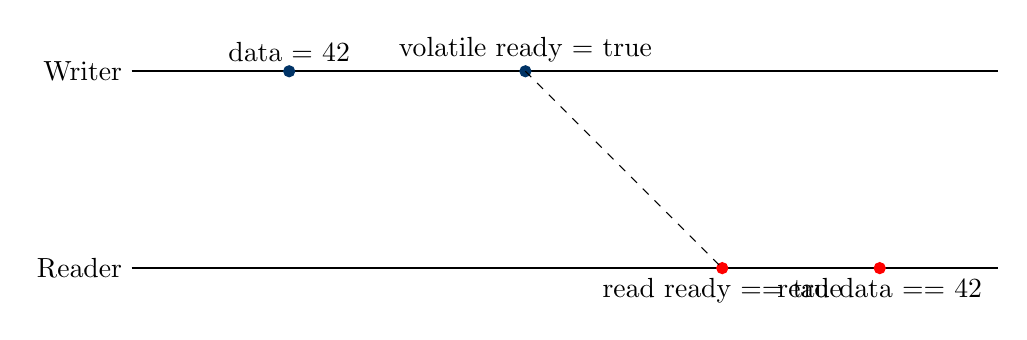
\begin{tikzpicture}[x=1cm,y=1cm]
			\draw[thick] (0,4) -- (11,4);
			\node[left] at (0,4) {Writer};
			
			\draw[thick] (0,1.5) -- (11,1.5);
			\node[left] at (0,1.5) {Reader};
			
			\filldraw[deepblue] (2,4) circle (2pt);
			\node[above] at (2,4) {data = 42};
			
			\filldraw[deepblue] (5,4) circle (2pt);
			\node[above] at (5,4) {volatile ready = true};
			
			\filldraw[red] (7.5,1.5) circle (2pt);
			\node[below] at (7.5,1.5) {read ready == true};
			
			\filldraw[red] (9.5,1.5) circle (2pt);
			\node[below] at (9.5,1.5) {read data == 42};
			
			\draw[dashed] (5,4) -- (7.5,1.5);
		\end{tikzpicture}
		
		\vspace{0.35cm}
		
		\begin{block}{Interpretation}
			The volatile flag acts as the communication gateway that carries visibility and ordering effects.
		\end{block}
	\end{frame}
	
	% =========================================================
	\begin{frame}{Enter Happens-Before}
		\begin{block}{Practical definition}
			If action A \textbf{happens-before} action B, then B is guaranteed to observe the effects of A in the way defined by the Java Memory Model.
		\end{block}
		
		\vspace{0.3cm}
		
		This is one of the most important ideas in Java concurrency.
		
		\vspace{0.3cm}
		
		\begin{exampleblock}{Think of it as}
			Not simply \emph{earlier in clock time}, but  
			\emph{earlier with a guaranteed memory relationship}.
		\end{exampleblock}
	\end{frame}
	
	% =========================================================
	\begin{frame}{Clock Time Is Not Enough}
		\begin{alertblock}{Common misconception}
			Students often think:
			\begin{quote}
				If A happened first in real time, then B must see it.
			\end{quote}
		\end{alertblock}
		
		\vspace{0.3cm}
		
		That is false in concurrent systems.
		
		\vspace{0.3cm}
		
		\begin{block}{Correct statement}
			What matters is not only temporal order, but whether the program established a valid \textbf{happens-before} relation.
		\end{block}
		
		\vspace{0.25cm}
		
		\begin{exampleblock}{Why this matters}
			Two actions may be separated in time and still lack the visibility guarantee needed for correct communication.
		\end{exampleblock}
	\end{frame}
	
	% =========================================================
	\begin{frame}{Important Happens-Before Rules}
		Some key practical rules are:
		
		\begin{itemize}
			\item A write to a volatile variable happens-before a later read of that same variable
			\item A call to \texttt{Thread.start()} happens-before actions in the started thread
			\item All actions in a thread happen-before another thread successfully returns from \texttt{join()}
			\item Unlocking a monitor happens-before a later lock of that same monitor
		\end{itemize}
		
		\vspace{0.3cm}
		
		\begin{exampleblock}{Connection to Week 3}
			We are not re-teaching locks here, but note that lock/unlock also establish memory guarantees.
		\end{exampleblock}
	\end{frame}
	
	% =========================================================
	\begin{frame}[fragile]{Volatile Happens-Before Example}
		\begin{lstlisting}
			class HbExample {
				static int value = 0;
				static volatile boolean published = false;
				
				public static void main(String[] args) {
					Thread writer = new Thread(() -> {
						value = 99;
						published = true;
					});
					
					Thread reader = new Thread(() -> {
						while (!published) {
						}
						System.out.println(value);
					});
					
					reader.start();
					writer.start();
				}
			}
		\end{lstlisting}
		
		\vspace{0.2cm}
		
		\begin{block}{Reasoning}
			The write to \texttt{published} happens-before the reader's later successful read of \texttt{published}.
		\end{block}
	\end{frame}
	
	% =========================================================
	\begin{frame}{What Happens-Before Gives You Here}
		In the previous example, once the reader observes:
		
		\[
		\texttt{published == true}
		\]
		
		it is not just seeing the flag itself.
		
		\vspace{0.3cm}
		
		It is also guaranteed to see the relevant earlier writes that logically preceded that volatile write, including:
		
		\[
		\texttt{value = 99}
		\]
		
		\vspace{0.3cm}
		
		\begin{alertblock}{This is the power of happens-before}
			It provides a defined memory relationship, not just a guessed runtime ordering.
		\end{alertblock}
	\end{frame}
	
	% =========================================================
	\begin{frame}{volatile as a Communication Signal}
		A useful student mental model is:
		
		\begin{center}
			\Large
			``ordinary data'' + ``volatile signal''
		\end{center}
		
		\vspace{0.3cm}
		
		\begin{exampleblock}{Pattern}
			\begin{itemize}
				\item write ordinary shared state first
				\item then write a volatile flag
				\item another thread reads the volatile flag
				\item then safely consumes the prepared state
			\end{itemize}
		\end{exampleblock}
		
		\vspace{0.3cm}
		
		\begin{block}{This is not universal thread safety}
			It is a very specific pattern for controlled communication.
		\end{block}
	\end{frame}
	
	% =========================================================
	\begin{frame}{What volatile Is Good For}
		Typical good uses include:
		
		\begin{itemize}
			\item stop flags
			\item readiness flags
			\item publication indicators
			\item one-writer / many-reader visibility patterns
			\item simple state variables where no compound action is required
		\end{itemize}
		
		\vspace{0.35cm}
		
		\begin{exampleblock}{Engineering rule}
			Use \texttt{volatile} when the main problem is:
			\begin{quote}
				``Other threads must see this update correctly.''
			\end{quote}
			not when the problem is:
			\begin{quote}
				``Several steps must behave as one indivisible unit.''
			\end{quote}
		\end{exampleblock}
	\end{frame}
	
	% =========================================================
	\begin{frame}{What volatile Is Bad For}
		Do not use \texttt{volatile} as if it solved:
		
		\begin{itemize}
			\item incrementing a shared counter safely
			\item protecting a check-then-act sequence
			\item safely updating multiple variables as one transaction
			\item replacing locks in all designs
		\end{itemize}
		
		\vspace{0.35cm}
		
		\begin{alertblock}{Common student mistake}
			They see ``shared variable'' and immediately think:
			\[
			\texttt{make it volatile}
			\]
			That is often incomplete or wrong.
		\end{alertblock}
	\end{frame}
	
	% =========================================================
	\begin{frame}[fragile]{The Famous Trap: volatile Counter}
		\begin{lstlisting}
			class VolatileCounter {
				static volatile int counter = 0;
				
				static void increment() {
					counter++;
				}
			}
		\end{lstlisting}
		
		\vspace{0.2cm}
		
		\begin{alertblock}{Question}
			Why is this still unsafe?
		\end{alertblock}
	\end{frame}
	
	% =========================================================
	\begin{frame}[fragile]{Why \texttt{counter++} Is Not Atomic}
		The statement
		
		\[
		\texttt{counter++}
		\]
		
		is not one indivisible action. Conceptually, it is:
		
		\begin{lstlisting}
			int temp = counter;
			temp = temp + 1;
			counter = temp;
		\end{lstlisting}
		
		\vspace{0.3cm}
		
		Two threads can interleave these steps and lose updates.
		
		\vspace{0.3cm}
		
		\begin{exampleblock}{Key point}
			Even if each read and write is visible, the \emph{whole update} is still a multi-step race.
		\end{exampleblock}
	\end{frame}
	
	% =========================================================
	\begin{frame}{Visibility Does Not Equal Atomicity}
		\begin{columns}[T]
			\column{0.48\textwidth}
			\begin{block}{Visibility question}
				Did thread B see thread A's latest write?
			\end{block}
			
			\column{0.48\textwidth}
			\begin{block}{Atomicity question}
				Did the update behave as one indivisible operation?
			\end{block}
		\end{columns}
		
		\vspace{0.35cm}
		
		\begin{alertblock}{Critical distinction}
			\texttt{volatile} helps with the left question.  
			It does not solve the right question.
		\end{alertblock}
		
		\vspace{0.25cm}
		
		\begin{exampleblock}{This is why Part 3 exists}
			Next we will separate visibility problems from atomicity problems more sharply.
		\end{exampleblock}
	\end{frame}
	
	% =========================================================
	\begin{frame}{A Comparison Slide}
		\centering
		\begin{tabular}{>{\bfseries}m{2.8cm} >{\centering\arraybackslash}m{2cm} >{\centering\arraybackslash}m{2cm} >{\centering\arraybackslash}m{2cm}}
			\toprule
			Mechanism & Visibility & Ordering & Atomicity \\
			\midrule
			Plain field & No guarantee & No guarantee & No guarantee for compound action \\
			\texttt{volatile} & Yes & Yes & No \\
			\texttt{synchronized} / lock & Yes & Yes & Yes for protected critical section \\
			\bottomrule
		\end{tabular}
		
		\vspace{0.4cm}
		
		\begin{exampleblock}{Why this slide matters}
			Students must stop treating all concurrency tools as interchangeable.
		\end{exampleblock}
	\end{frame}
	
	% =========================================================
	\begin{frame}[fragile]{Another Practical Example: Configuration Publication}
		\begin{lstlisting}
			class ConfigDemo {
				static String config;
				static volatile boolean loaded = false;
				
				public static void main(String[] args) {
					Thread loader = new Thread(() -> {
						config = "MODE=SAFE";
						loaded = true;
					});
					
					Thread user = new Thread(() -> {
						while (!loaded) {
						}
						System.out.println(config);
					});
					
					user.start();
					loader.start();
				}
			}
		\end{lstlisting}
		
		\vspace{0.2cm}
		
		\begin{block}{Use case}
			Prepare ordinary data, then publish readiness through a volatile flag.
		\end{block}
	\end{frame}
	
	% =========================================================
	\begin{frame}{When volatile Is Elegant}
		\begin{exampleblock}{Elegant case}
			A thread prepares a result once, then tells other threads:
			\[
			\texttt{``It is ready now.''}
			\]
		\end{exampleblock}
		
		\vspace{0.3cm}
		
		This is where \texttt{volatile} shines:
		\begin{itemize}
			\item simple
			\item efficient
			\item no lock-based waiting needed for the flag itself
		\end{itemize}
		
		\vspace{0.3cm}
		
		\begin{alertblock}{But elegance has limits}
			As soon as your correctness depends on a multi-step shared update, \texttt{volatile} alone is usually not enough.
		\end{alertblock}
	\end{frame}
	
	% =========================================================
	\begin{frame}{Common Misconceptions to Kill Early}
		Students should \textbf{not} leave this lecture thinking:
		
		\begin{itemize}
			\item ``volatile means thread-safe''
			\item ``volatile is a lighter lock''
			\item ``volatile fixes every shared variable problem''
			\item ``if a value is visible, then increments are safe''
		\end{itemize}
		
		\vspace{0.35cm}
		
		\begin{alertblock}{Replace with}
			\begin{quote}
				\texttt{volatile} is a tool for visibility and ordering of shared communication, not a general solution for compound shared-state correctness.
			\end{quote}
		\end{alertblock}
	\end{frame}
	
	% =========================================================
	\begin{frame}{Part 2 Concept Summary}
		\centering
		\begin{tabular}{>{\bfseries}m{3cm} m{7.3cm}}
			\texttt{volatile} & special shared field with visibility and ordering guarantees \\
			Visibility & later reads can observe the written value correctly \\
			Ordering & earlier writes become meaningful relative to the volatile signal \\
			Happens-before & formal guarantee relation between memory actions \\
			Good use & flags, readiness, publication \\
			Limitation & no compound atomicity \\
		\end{tabular}
	\end{frame}
	
	% =========================================================
	\begin{frame}{Lab Preparation for Part 2}
		\begin{block}{Lab 4.2 --- Fix the Stop Flag}
			Students convert an unsafe stop flag into a volatile stop flag.
		\end{block}
		
		\vspace{0.25cm}
		
		\begin{block}{Lab 4.3 --- Publication with a Volatile Flag}
			Students publish ordinary data using:
			\begin{itemize}
				\item data field
				\item volatile ready flag
			\end{itemize}
		\end{block}
		
		\vspace{0.25cm}
		
		\begin{block}{Lab 4.4 --- Volatile Counter Failure}
			Students test a volatile counter under repeated increments and explain why the result is still wrong.
		\end{block}
	\end{frame}
	
	% =========================================================
	\begin{frame}{Suggested Discussion Questions}
		\begin{enumerate}
			\item Why does \texttt{volatile} fix the stop flag?
			\item Why is \texttt{volatile} useful for publication patterns?
			\item What is the difference between seeing a value and updating safely?
			\item Why is clock time not enough to reason about memory visibility?
			\item Why does \texttt{counter++} remain unsafe even when \texttt{counter} is volatile?
		\end{enumerate}
	\end{frame}
	
	% =========================================================
	\begin{frame}{Takeaway}
		\begin{alertblock}{Final takeaway for Part 2}
			\texttt{volatile} allows threads to communicate through a variable with defined visibility and ordering semantics.
		\end{alertblock}
		
		\vspace{0.35cm}
		
		\begin{block}{But}
			It does \emph{not} make compound shared-state operations atomic.
		\end{block}
		
		\vspace{0.35cm}
		
		\begin{exampleblock}{Bridge to Part 3}
			Now that we know how visibility can be fixed, the next question is:
			
			\begin{center}
				\Large
				Why can a program still be wrong even when visibility is correct?
			\end{center}
		\end{exampleblock}
		
		\vspace{0.2cm}
		
		That leads directly to:
		\[
		\textbf{visibility vs atomicity}
		\]
		and
		\[
		\textbf{broken double-checked locking}
		\]
	\end{frame}
	
	% =========================================================
	\begin{frame}{End of Part 2}
		\centering
		\Huge Questions?
	\end{frame}
	
	% =========================================================
\end{document}